\documentclass[../main.tex]{subfiles}
	% ELECTRONICS TESTING
\begin{document}

The assessment of the electronic capabilities of the test bed is split into three main sections.
The first section deals with the electircal characteristics of the Raspberry Pi and pertains to the GPIO pins and their physical capabilities.
The second section deals with the computational characteristics of the Raspberry Pi, and particularly how fast the pin values can be changed and read by the underlying code, and how most efficiently to achieve this.
The third section deals with the components used in the test bed, discussing limitations to its operation which are posed by the components used.\\

%%%%%%%%%%%%%%%%%%%%%%%%%%%%%%%%%%%%%%%%%%%%%%%%%%%%%%%%%%%%%%%%%%%%%%%%%%%%%%%%%%%%%%%%%%%%%%%%%%%%%%%%%%%%%%%%%%%%%%%%%%%%%%%%%%

\section{Electrical Characteristics of the Raspberry Pi}

The Raspberry Pi 3 Model B+ has 40 pins, including eight ground pins, two \SI{3.3}{\volt} power pins and two \SI{5}{\volt} power pins.
26 of the remaining pins (BCM pins 2 to 27) are free to be used as General Purpose Input/Output (GPIO).
The GPIO pins can output low (\SI{0}{\volt}) and high (\SI{3.3}{\volt}) levels, and they are powered by the same \SI{3.3}{\volt} rail as the power pins of the same voltage.
As a result, there is a maximum current that can be drawn from all of these pins together as well as from each GPIO pin individually.\\

The Embedded Linux Wiki claims that the \SI{5}{\volt} pins can provide a maximum current equal to, "The USB [power cable] input current (usually \SI{1}{\ampere}) minus any current draw from the rest of the board." \cite{web_RpiMaxRatings}
It also provides the maximum current to be drawn from all \SI{3.3}{\volt} power pins as \SI{50}{\milli\ampere} (this would apply to the power pins and the GPIO pins combined).
However that specification was actually a design value for the original Pi, designed to supply \SI{3}{\milli\ampere} for each of its17 pins for $\approx \SI{51}{\milli\ampere}$ total, according to Gert Van Loo, the hardware engineer of the first Pi's boards \cite{web_RPiSpecsSE}.
There is nothing limiting the current-output on the pins, so they will attempt to drive whatever current is drawn until they stop working.
However, multiple sources including Gert Van Loo suggest that the maximum current that should be drawn from any one pin for safe operation is \SI{16}{\milli\ampere} as this is the current to which the electronics on each pad are rated.
Mosaic Documentation Web also has a page attempting to define the electrical specifications of the Raspberry Pi \cite{web_MosaicSpecs}, and it also suggests that one should not attempt to source or sink more than \SI{16}{\milli\ampere} on an output pin.
The pins actually have a set drive strength from \SIrange{2}{16}{\milli\ampere} in \SI{2}{\milli\ampere} increments which is set for a bank of pins and usually set to \SI{8}{\milli\ampere} but even a pin set to \SI{2}{\milli\ampere} drive strength and then loaded so as to draw \SI{16}{\milli\ampere} will not be damaged \cite{web_GPIOPadsErrata}.\\

The maximum current which can be drawn from an output pin is a useful detail.
This is used to ensure that none of the attached components draw too much current.
It is also used to decide, along with the input impedances of the pins, whether or not the GPIO pins of one Raspberry Pi can be connected directly to another without a protective resistor between them.
It is important that the ground pins of the two Raspberry Pis be connected together so that they share a common reference for the data levels.
The input and output impedances of the pins in various set-up modes are shown in Table \ref{tab_Pin Impedances}.
All values were measured on a multi-meter and using the pin GPIO26 (and compared to other pins to check consistency).
Pins 2 and 3 have permanent internal pull-up resistors whereas all of the rest have software-controllable pull-up or pull-down resistors which can be set for inputs.\\

\begin{table}[h]
	\centering
	\global\tabulinesep = 2mm
	\begin{tabu} to 0.8\textwidth { | X[l] | X[c] | }
		\hline
		Input/Output Mode & Impedance to Ground ($\SI{}{\kilo\ohm}$)\\
		\hline\hline
		Input & Open Loop\\
		\hline
		Input with Pull-Up Resistor  & 53 250\\
		\hline
		Input with Pull-Down Resistor  & 49.24\\
		\hline
		Output & 0.0329\\
		\hline
		Raspberry Pi ON (No Mode) & 49.23\\
		\hline
		Raspberry Pi OFF & 606.14\\
		\hline
	\end{tabu}
	\caption{Table of GPIO Pin Impedances for Different Operating Modes}
	\label{tab_Pin Impedances}
\end{table}

These impedances show that even the lowest input impedance of \SI{48.93}{\kilo\ohm} will only draw \SI{67.44}{\micro\ampere} of current from a \SI{3.3}{\volt} GPIO pin, and this is three orders of magnitude lower than the maximum current these pins can supply.
The impedance of pins set to be outputs is the only value lower than this at \SI{32.9}{\ohm}, and so if an output at \SI{0}{\volt} were connected to another pin at \SI{3.3}{\volt} it would potentially draw about \SI{100}{\milli\ampere} which would damage both pins or at least (the Raspberry Pi has safeguards excessive currents) restart the Pi.
However, this is unlikely to happen in the test bed setup unless an output pin is directly connected to a \SI{3.3}{\volt} power pin, or both Pis have directly connected pins set as outputs.
In conclusion, the pins of two Raspberry Pis can be directly connected together, as long as care is taken not to have both devices setting these pins to outputs at the same time .\\

%\clearpage

%%%%%%%%%%%%%%%%%%%%%%%%%%%%%%%%%%%%%%%%%%%%%%%%%%%%%%%%%%%%%%%%%%%%%%%%%%%%%%%%%%%%%%%%%%%%%%%%%%%%%%%%%%%%%%%%%%%%%%%%%%%%%%%%%%

\section{Computational Characteristics of the Raspberry Pi} \label{sec_Computation}

The Raspberry Pi is not a real-time device.
Running under an operating system, there will always be interrupts due to scheduling of different threads, which mean that code execution may not always be as perfectly timed as it would be on a dedicated embedded device like an Arduino.
The Raspberry Pi has certain advantages however; Python is significantly more versatile for signal processing, and the Raspberry Pi B+ has a \SI{1.4}{\giga\hertz} processor compared to the Arduino Uno's \SI{16}{\mega\hertz} clock \cite{lib_Arduino}.
There are also ways of ensuring the Pi operates as close to real time as possible.\\

The time-sensitive parts of the code are the actual pin manipulations in the transmitter, and the reading in of the pin values in the receiver.
This means that these need to be the parts optimised for speed.
System interrupts can be turned off in the code, however this results in nothing else being run on the computer, essentially freezing it until the interrupts are turned back on \cite{web_Interrupts}.
This should not be done for a long period of time as it is bad for the Pi, and in this case the transmitter and receiver may be used to transmit for a significant amount of time.
This means that disabling all interrupts is not a good idea without periodically turning on interrupts to allow them to run, and this would result in losing samples at the receiver to the backlog of interrupts.
However, there is one particularly inhibiting interrupt - adjusting of the refresh rate of RAM every 500ms - which can be turned off, and should be for any processor-intensive work \cite{web_PiOscilloscope}.
This is achieved with the terminal command in Listing \ref{lst_RAM Refresh}.\\

\lstset{style=C}
\begin{lstlisting}[caption={Turning off the RAM refresh rate adjustment}, label={lst_RAM Refresh}]
	sudo sed -i '$s/$/\ndisable_pvt=1/' /boot/config.txt
\end{lstlisting}

The choice to keep the common clock and carrier was to simplify the rest of the setup, after a number of attempts at synchronisation were made.
This becomes particularly important when dealing with carrier modulated signals as a phase-locked loop would be required to recover the phase of the carrier.
This decision is also made based on precedent -- the DIWINE project in their second White Paper, two years into a three year project, still describe a "'time zero' reference" between the terminal nodes of their test bed for synchronisation \cite{pap_DIWINEpaper2}.

\subsection{Comparing Python and C} \label{sec_Comparing Python and C}

Python is implemented as an interpreted language, meaning that the code (or at least an intermediate byte-code representation) is interpreted by a virtual machine at runtime.
This means that, although a lot more powerful, Python has drawbacks in performance relative to C, which is compiled into executable machine code prior to being run.
An article by Joonas Pihlajamaa from 2015 benchmarked the frequencies which could be achieved by switching a GPIO on and off continuously.
It suggests that the Python library RPi.GPIO achieved the highest frequency of the Python libraries, at \SI{70}{\kilo\hertz} \cite{web_BenchmarkingPi}.
It also suggests that all of the C libraries tested achieved frequency ranges in the Megahertz, although it did not benchmark \textit{pigpio} which this test bed uses.
The libraries have been updated to improve efficiency since 2015, but if C is found to be a significantly better option, then the pin manipulations of the transmitter and receiver themselves should be written in C and compiled into executables which the main Python code-base can run.\\

\begin{figure}[ht]
	\centering
	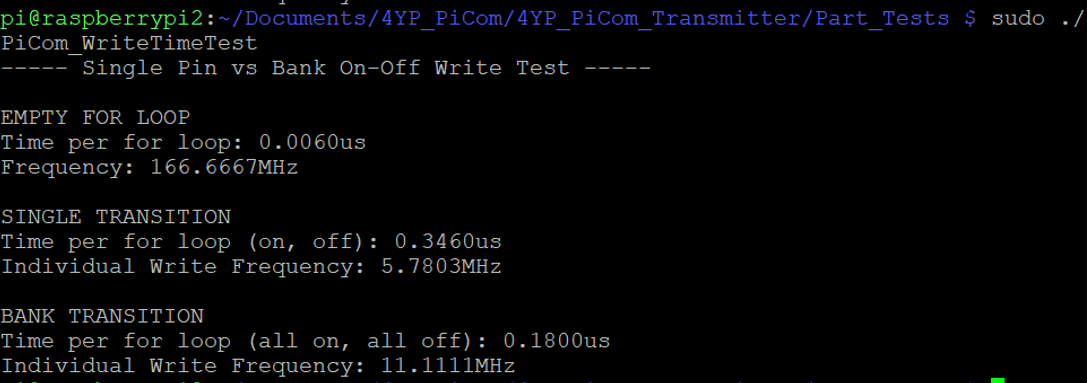
\includegraphics[width=\textwidth]{Write_Time_Test.png}
	\caption{Results of PiCom\textunderscore Write\textunderscore Time\textunderscore Test}
	\label{fig_Write Time Test}
\end{figure}

The test in the benchmarking article was performed with Python \textit{RPi.GPIO} and C \textit{pigpio}; an endless while loop writing a '1' then a '0' was started on a single pin, and the output frequency measured on an oscilloscope.
The result was conclusive: Python produced a clock frequency of about \SI{238}{\kilo\hertz}, whereas the C code produced a clock frequency of about \SI{2.87}{\mega\hertz}.
Having decided that the pin manipulations were to be done using \textit{pigpio} in C, the next step was to decide whether to use the bank read and write functions or the single-pin alternatives.
This may seem an obvious choice, but depending on the speed of the read functions in particular, it may be more efficient to read each pin individually into a global variable holding their values as they are updated than to read all of them at once.\\

The results comparing the single pin write and bank (setting eight values corresponding to the DAC mask) write functions are in Figure \ref{fig_Write Time Test}.
This test was done using the timer function \colorbox{backcolour}{\lstinline{gpioTick()}} to average over the time of 1000 iterations of a for loop.
An empty for loop is included for comparison.
Importantly, the single pin write loop consists of setting the pin on and then off, whereas a bank write consists of a bank clear and set, so the equivalent loop is clear 0 and set the DAC mask, followed by clear the DAC mask and then set 0.
Even though this is the case, the bank write is still approximately twice as fast as a single pin write, probably due to lower level direct memory access.
The bank write can also set all 8 or 16 DAC pins at once and so is the clear favourite.\\

\begin{figure}[ht]
	\centering
	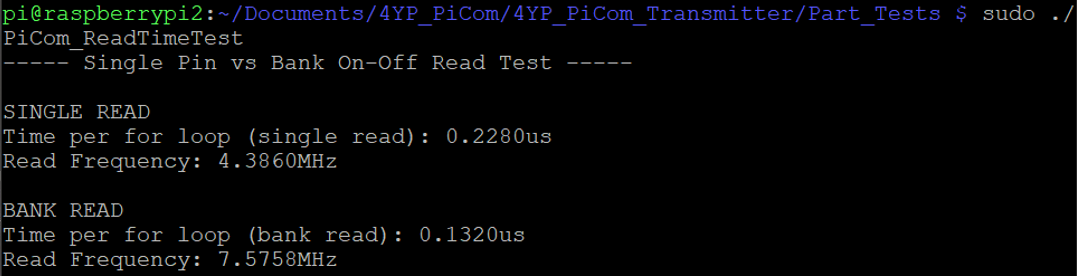
\includegraphics[width=\textwidth]{Read_Time_Test.png}
	\caption{Results of PiCom\textunderscore Read\textunderscore Time\textunderscore Test}
	\label{fig_Read Time Test}
\end{figure}

The results comparing the single pin read and bank read functions are in Figure \ref{fig_Read Time Test}.
This time there is only one function call in each loop, and again the bank function is about twice as fast.
This suggests that reading each pin individually is a waste of time, as even if this was required, the bank function could read all of the pins in less time.
As a result, all C code uses the bank functions except for the second (rising edge) clock transition in the transmitter which needs to happen after the DAC write and falling clock edge happen simultaneously in the bank write.

%%%%%%%%%%%%%%%%%%%%%%%%%%%%%%%%%%%%%%%%%%%%%%%%%%%%%%%%%%%%%%%%%%%%%%%%%%%%%%%%%%%%%%%%%%%%%%%%%%%%%%%%%%%%%%%%%%%%%%%%%%%%%%%%%%

\section{Characterising Components of the Test Bed} \label{sec_Components}

In order to use components in the test bed, it must be ensured that they are working correctly, such that any problems can be solved or mitigated.
As there are a large number of components available, it is possible that some may be unsuitable for the intended use or may not work exactly as expected, therefore it is important to ensure that all components are working correctly and performing appropriately prior to including them in the test bed.

\subsection{Digital Analogue Converter} \label{sec_Characterising DAC}

The Digital Analogue Converter uses a resistor ladder connected to $V_{ref}$ to determine the output.
Switches determined by the digital values latched at the input of the device connect the corresponding resistor to either $I_{out1}$ (the output) or $I_{out2}$ (which is connected to ground).
The ladder is designed such that each digital bit corresponds to a voltage twice the value of the bit before it is switched to the output, therefore giving an output proportional to the digital input value.
In order to confirm that this is indeed the case, the transmitter is run with 256PAM modulation with an input of monotonically increasing byte values 0 to 255 repeating.
This should ideally produce a monotonic linear output.
Figure \ref{fig_DAC Non-continuous} shows the output of the DAC, with the output on probe 1 (yellow) and the data value of \SI{3.3}{\volt} on probe 2 (green).\\

\begin{figure}[ht]
	\centering
	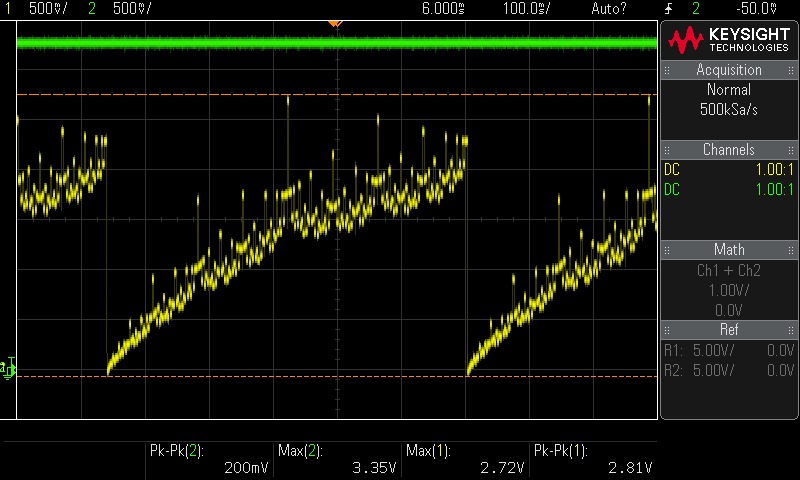
\includegraphics[width=0.8\textwidth]{Screen_256PAM.png}
	\caption{DAC non-linearly increasing output voltage for linearly increasing digital input values}
	\label{fig_DAC Non-continuous}
\end{figure}

The output is clearly not as expected which represents an unfortunate shortcoming if not rectified.
The values seem to jump around the general trend expected, with peaks particularly at values of 64, 128 and 192.
Decoupling the output from the power supply was attempted but this did nothing to affect the output, and lab technicians were consulted to no avail.
The program was rerun with a pause point in the code between each output value to confirm that this behaviour was not to do with the output frequency, to verify that the bitmasks were giving the correct digital outputs (which they were), and to check that the peak points were the aforementioned values, corresponding to binary inputs of $0b01000000$, $0b10000000$ and $0b11000000$ respectively (where $0b$ signifies the binary representation).
The behaviour is also consistent for both of the DACs purchased.\\

\begin{figure}[ht]
	\centering
	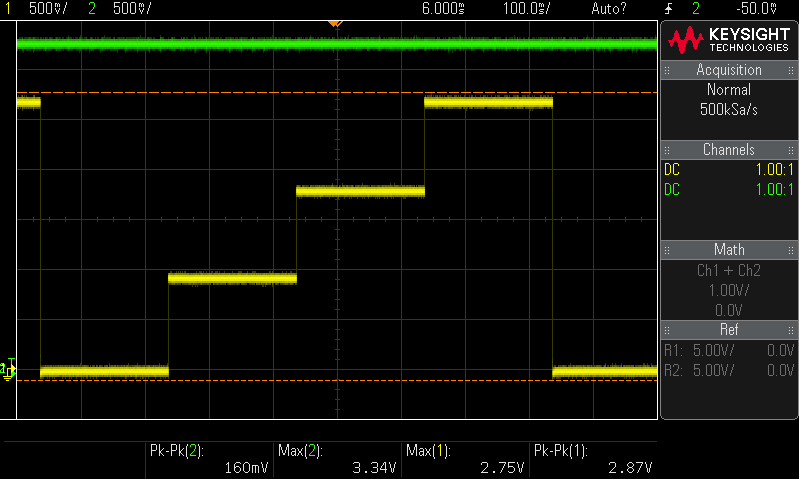
\includegraphics[width=0.6\textwidth]{Screen_4PAM.png}
	\caption{4PAM output with lookup table}
	\label{fig_4PAM Lookup}
\end{figure}

The solution chosen for this problem was to use a lookup table for empirical digital values which as closely as possible correspond to equidistant output values.
This lookup table is used in the code to translate each PAM symbol or the real and imaginary parts of each QAM symbol from the range $[0, 3]$ to particular digital values, rather than as previously simply multiplying by 85 to produce values from $0$ to $255$.
Figure \ref{fig_4PAM Lookup} shows the output of 4PAM with such a table.
Values are close, but there are some slight discrepancies, and this lookup takes advantage of the 128 maximum peak for larger output range but this could be dangerous if either DAC stopped exhibiting this peak for some reason.

\subsection{Analogue Digital Converter}

For the Analogue Digital Converter, the conversion is not instantaneous; it contains a DAC, a series of dividers and a comparator, and is constantly comparing the most significant bit (MSB) to $\frac{V_{ref}}{2}$ while $\overline{WR}$ is low.
When the trigger goes high the conversion starts, and runs for eight clock pulses of the ADC's internal clock.
On completion of this conversion the $\overline{BUSY}$ pin goes high, which is taken as the read clock for the receiver Raspberry Pi.
The sampled output of a 5Hz wave sampled 5000 times at \SI{10}{KSPS} is shown in Figure \ref{fig_ADC Input} with the expected value shown in red underneath the data, plotted with matplotlib \cite{lib_matplotlib}.
The output has periods where it stops following the input signal and settles at the middle value instead but other than that follows the values fairly accurately.\\

\begin{figure}[ht]
	\centering
	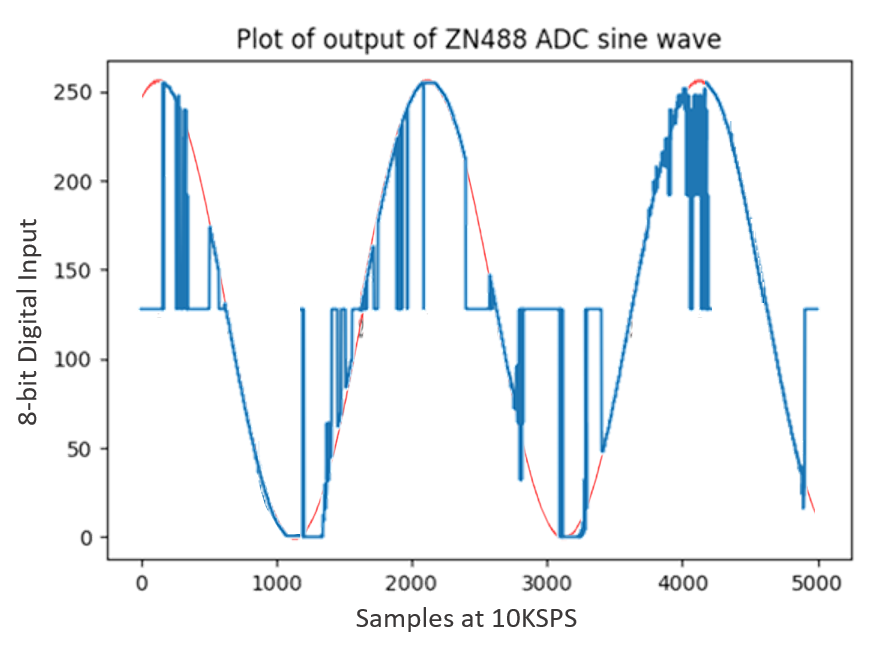
\includegraphics[width=0.6\textwidth]{ADC_sine_output.png}
	\caption{Input of ADC for a 5Hz sine wave generated with a signal generator}
	\label{fig_ADC Input}
\end{figure}

It was originally thought that the ADC is on occasion jumping to the added DC value of the zero-centred sine wave, but it is also possible that it is occasionally missing timing and sampling during the time when the $\overline{WR}$ pin is low and the output is set to $0b10000000$ to compare the most significant bit.
This data was collected when the write clock signal from the transmitter (on the $\overline{WR}$ pin of the ADC) was positive for $50\%$ of the clock cycle and 0 for $50\%$, but it was realised that a more logical signal for the operation of both converters is a small falling edge then rising edge pulse to latch the data in the DAC and to start the conversion of the ADC.
If the problem was the DC value it will not affect the test bed, and if it was the delayed timing then the adjusted clock signal should make this far less likely.
Unfortunately it was not possible to collect new data to verify this due to time constraints with the signal generator.

\subsection{Quadrature Pulse Generator}

The chip used to generate the sine waves is a quadrature pulse generator, outputting two square waves $90^o$ out of phase.
Frequency output can be in the range \SIrange{5}{1100}{\kilo\hertz}.
Figure \ref{fig_Pulse Output} shows the output of the pulse generator for resistor values of \SI{1}{\mega\ohm} (\SI{100}{\kilo\hertz}) and \SI{100}{\kilo\ohm} (\SI{1}{\mega\hertz}) respectively.

\begin{figure}[ht]
	\centering
	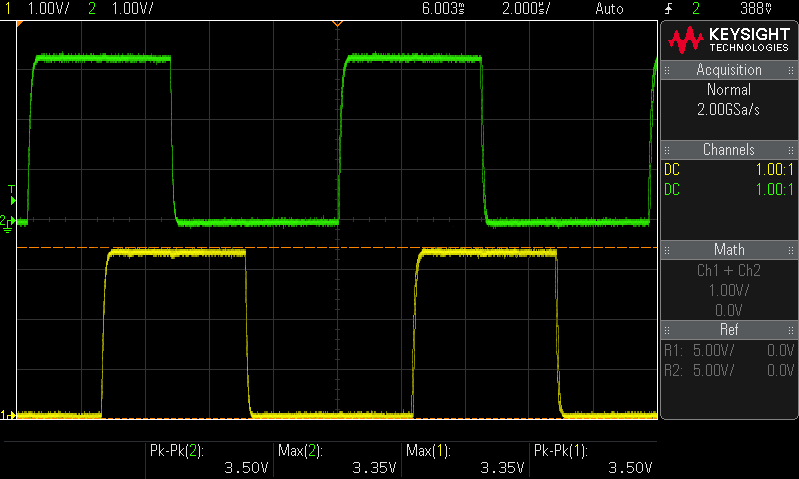
\includegraphics[width=0.49\textwidth]{Screen_1MOhm.png}
	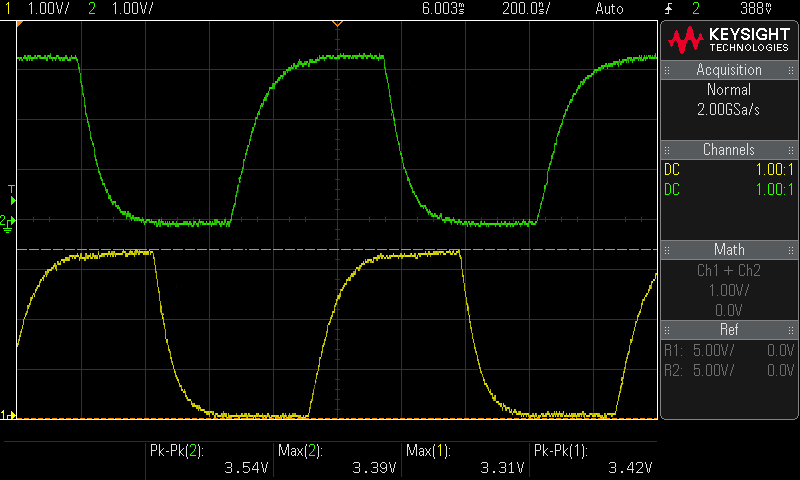
\includegraphics[width=0.49\textwidth]{Screen_100kOhm.png}
	\caption{Output of quadrature pulse generator at 100kHz (left) and 1MHz (right)}
	\label{fig_Pulse Output}
\end{figure}

A single carrier frequency needs to be selected in order to design the low pass filters used to convert the square wave outputs into phase-shifted sine waves.
A frequency of \SI{100}{\kilo\hertz} was chosen as the wave form was a lot more stable at this frequency, but this is a design choice.
Figure \ref{fig_ADC Sine} shows the same outputs filtered with a second order passive RC filter.

\begin{figure}[ht]
	\centering
	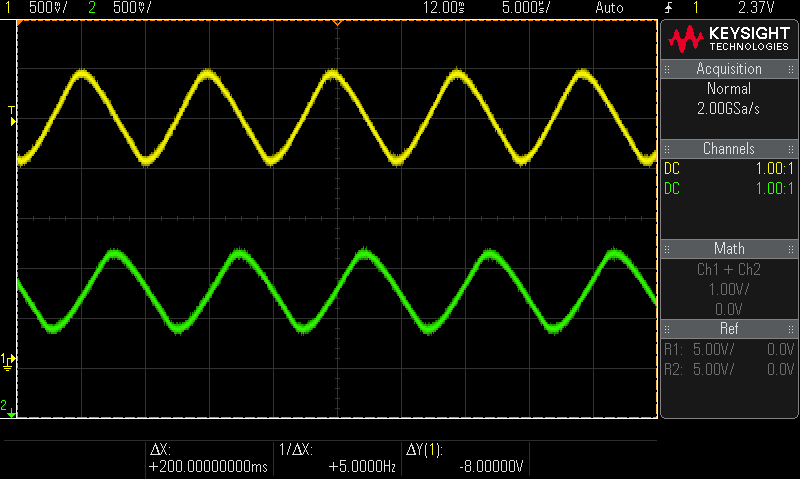
\includegraphics[width=0.6\textwidth]{Screen_Sine_Output.png}
	\caption{Output of pulse generator once filtered to be sine waves}
	\label{fig_ADC Sine}
\end{figure}

\subsection{Overdriving Component Clocks} \label{sec_Overclocking}

The \textit{pigpio} library has access to the hardware clocks of the Raspberry Pi.
Specifically on the Pis used, it has the ability to set a hardware clock which is not reserved for system use to a specified frequency between \SI{4.7}{\kilo\hertz} and \SI{250}{\mega\hertz} on pin 4, although the library documentation suggests that frequencies above \SI{30}{\mega\hertz} are unlikely to work \cite{lib_pigpioHWClock}.\\

\begin{figure}[ht]
	\centering
	%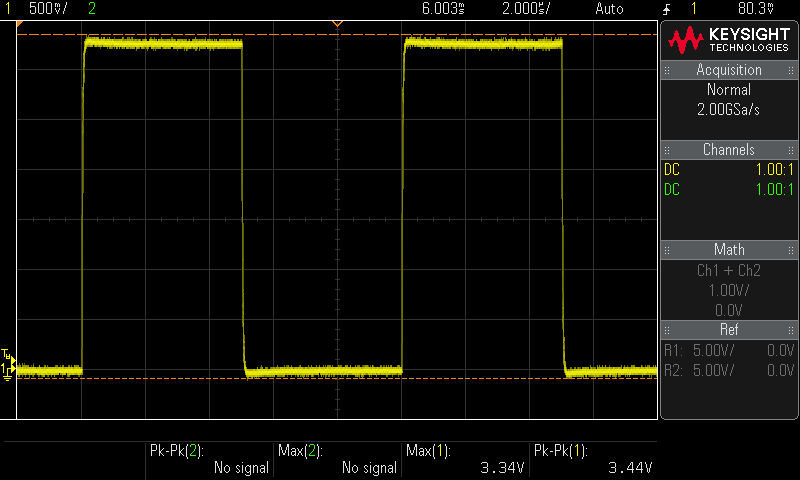
\includegraphics[width=0.4\textwidth]{Screen_100kHz.png}
	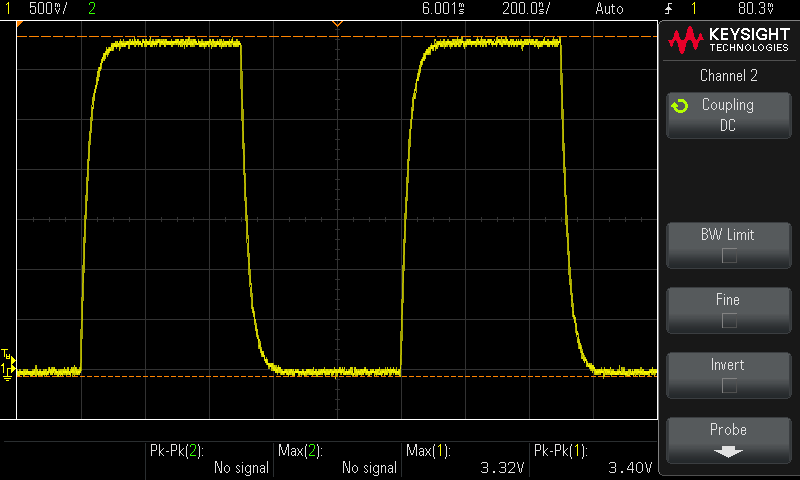
\includegraphics[width=0.6\textwidth]{Screen_1MHz.png}
	\caption{A 1MHz clock signal produced by the hardware clock}
	\label{fig_HWClock}
\end{figure}

There are certain components which work using an internal clock set by an external resistor or capacitor, but which may be overdriven by an external clocking signal, and this functionality may be used.
This would allow the frequencies of these devices to be defined in software with less reliance on external physical components.
This is particularly relevant for the Analogue Digital Converter as it requires eight clock pulses per conversion, and setting a hardware clock for (at least) eight times the transmission frequency is one way of ensuring this in software.
Figure \ref{fig_HWClock} shows the stability of this hardware clock at \SI{1}{\mega\hertz} which is the maximum clocking frequency of the ADC.\\

\end{document}